\documentclass[11pt]{article}
\usepackage{multicol}
\usepackage{ifthen}
%\usepackage{multitoc}
%\usepackage{german}
%\usepackage{bibgerm}
\usepackage{amsthm}
\usepackage{amsmath}
\usepackage{amsfonts}
\usepackage{color}
\usepackage{hyperref}
\usepackage[dvips]{epsfig}
\usepackage[dvips]{graphicx}
\usepackage[a4paper,body={148mm,240mm,nohead}]{geometry}
\usepackage[ansinew]{inputenc}
\usepackage{listings}
\lstset{language=C++, basicstyle=\ttfamily,
  stringstyle=\ttfamily, commentstyle=\it, extendedchars=true}

\newif\ifpdf
\ifnum\ifx\pdfoutput\undefined0\else\pdfoutput\fi<1
\pdffalse % we are not running PDFLaTeX
\else
\pdftrue % we are running PDFLaTeX
\fi

\ifpdf
\usepackage[pdftex]{graphicx}
\else
\usepackage{graphicx}
\fi

\ifpdf
\DeclareGraphicsExtensions{.pdf, .jpg, .tif}
\else
\DeclareGraphicsExtensions{.eps, .jpg}
\fi

%\theoremstyle{plain}
\newtheorem{theorem}{Theorem}[section]
\newtheorem{lemma}[theorem]{Lemma}

\theoremstyle{definition}
\newtheorem{definition}[theorem]{Definition}
\newtheorem{class}[theorem]{Class}
\newtheorem{algorithm}[theorem]{Algorithm}
\theoremstyle{remark}
\newtheorem{remark}[theorem]{Remark}

\newcommand{\C}{\mathbb{C}}
\newcommand{\R}{\mathbb{R}}
\newcommand{\N}{\mathbb{N}}
\newcommand{\Z}{\mathbb{Z}}
\newcommand{\Q}{\mathbb{Q}}
\newcommand{\K}{\mathbb{K}}
\newcommand{\loc}{\mbox{loc}}

\title{Communication within the Iterative Solver Template Library (ISTL)\thanks{Part of the
    Distributed and Unified Numerics Environment (DUNE) which is
    available from the site
    \texttt{http://www.dune.uni-hd.de/}}}

\author{%
Markus Blatt\\
Interdisziplin�res Zentrum f�r Wissenschaftliches Rechnen,\\
Universit�t Heidelberg, Im Neuenheimer Feld 368, D-69120 Heidelberg, \\
email: \texttt{Markus.Blatt@iwr.uni-heidelberg.de}}

\date{April 27, 2005}

\begin{document}

\maketitle

\begin{abstract}
  This document describes usage and interface of the classes meant for
  setting up the communication within a parallel programm using
  ISTL. As most of the communication in distributed programm occur in
  the same pattern it is often more efficient (and of course more easy
  for the programmer) to build the communication pattern once in the
  programm and then use multiple times (e.~g. at each iteration step
  of an iterative solver).
\end{abstract}

\begin{multicols}{2}
{\small\tableofcontents}
\end{multicols}


\section{Introduction}
\label{sec:introduction}


\section{Index Sets}
\label{sec:index-sets}

During distributed computations every discretization point needs to be
indentified uniquely by every process regardless of where it is
actually stored. In most scenarios it not advisable to store all the
data needed for the computation on every process as memory is often a
limiting factor in scientific computing. Therefore the data will
distributed between the processes and each process will store only the
data corresponding to its own part of the distribution. Due to the
efficiency of the local commnunication is it normally best practice to
hold the locally stored data in consecutive memory chunks.

This means that for the local computation the data must be adressable
by a consecutive index starting from 0. When using adaptive
discretization methods there might be need to reorder the indices
after adding and/or deleting some of the discretization
points. Therefore this index does not have to be persistent. Further
on  we will call this index {\em\index{local index}local index}.

For the communication phases of our algorithms these locally stored
indices must also be adressable by a global identifier to be able to
store the received values tagged with the global identifiers at the
correct local index in the consecutive local memory chunk. To ease the
addition and removal of discretization points this global identifier has
to be persistent. Further on we will call this global identifier
{\em\index{global index}global index}.

\paragraph{IndexSet}
  Let $I \subset \N_0$ be an arbitrary, not necessarily consecutive,
  index set identifying all discretization points of the computation.
  
  Further more let $(I_p)_{p\in[0,P)}$, 
  $\bigcup\limits_{p=0}^{P-1} I_p = I$ be an overlapping decompostion of the global index set
  $I$ into the sets of indices $I_p$ corresponding to the
  discretization points stored locally on process $p$.

  Then the 
  \begin{lstlisting}{}
    template<typename TG, typename TL, int N> 
    class IndexSet;
  \end{lstlisting} 
  realizes the one to one mapping 
  $$
  \gamma_p\::\: I_p \longrightarrow I^{\loc}_p := [0, n_p)
  $$
  of the globally unique index onto the local index. 

  The template parameter \lstinline!TG! is the type of the global
  index and
  \lstinline!TL! is the type of the local index, that has to be
  convertible to \lstinline!std::size_t!, and the parameter
  \lstinline!N! is used internally to specify the chunk size of the
  array list.

The pairs of global and local index are ordered by ascending global
index. Thus it it possible to access the pairs via
\lstinline!operator[](TG& global)! in $log(n)$ time, where $n$ is the
number of pairs in the set.

Due to the ordering the index set can only be changed, i.~e. indices
added or deleted, in a special resize phase. By calling the functions
\lstinline!beginResize()! and \lstinline!endResize()! the programmer
indicates that the resize phase starts and ends, respectively. During
the call of \lstinline!endResize()! the deleted indices will be
removed and the added indices will be merged with the existing
ones.

To be able to attach further information to the index the only
prerequesite for the type of the local index is that it is convertible
to \lstinline!std::size_t! as it it meant for adressing array
elements.

\paragraph{ParallelLocalIndex}
When dealing with overlapping index sets in distributed computing
there often is the need to distinguish different part of the index
set, e.~g. mark some of the indices as owned by the process and others
as owned by another process.

This can easily be done by using the class
\begin{lstlisting}{}
  template<typename TA>
  class ParlallelLocalIndex;
\end{lstlisting}
where the template parameter \lstinline!TA! is the type of the
attributes used, e.~g. \lstinline!enum{owner, overlap}!.

As the programmer often knows in advance which indices might also be
present on other processes there is the possiblity to mark the index
as public.

\paragraph{Usage Examples}
Let us look at a short example on how to build an index set. The code
in Listing \ref{lst:build_indexset} sets up an index set with 8
components on two processes. This index set might be used to access as
distributed field or \lstinline!std::vector! as sketched in Figure
\ref{fig:distributed_field}. 

\begin{figure}[htb]
  \centering
  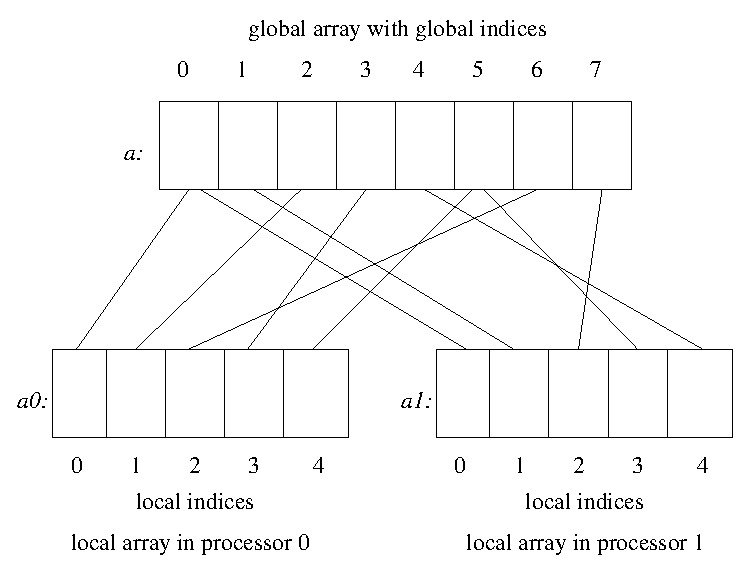
\includegraphics{figures/darray.eps}
  \caption{A Distributed Field}
  \label{fig:distributed_field}
\end{figure}

The process $0$ stores in his {/em local}
field $a_0$ the values corresponding to the global indices
$I_0=\{0,2,6,3,5\}$, in that order, of the global field $a$ and process
$I$ the entries corresponding to the values at the indices
$I_1=\{0,1,7,5,4\}$.
\lstinputlisting[caption=Build an Index Set,
label=lst:build_indexset]{buildindexset.hh}

Due to the complexity of \lstinline!operator[](TG& global)! it is
always advisable to use iterators, obtained by calling
\lstinline!begin()! and \lstinline!end()! respectively, to access the
index pairs of the set.

Listing \ref{lst:indexset_iterator} demonstrates their
usage. First the maximum local index $i_{\mbox{max}}$ of the set is
computed, and the 
the local indices are renumbered. Due to the ordering the local index with
the smallest corresponding global index becomes $i_{\mbox{max}}$ and the rest is
numbered consecutively decreasingly with increasing global index. Let
$n$ be the number of index pairs in the set than local index
corresponding to the largets global index becomes $i_{\mbox{max}}-n$.
\lstinputlisting[caption=Usage of Index Set Iterators,
label=lst:indexset_iterator]{reverse.hh}

\section{Remote Indices}
\label{sec:remote-indices}


\section{Communication Interface}
\label{sec:comm-interf}


\section{Communicator}
\label{sec:communicator}



\end{document}
%%% Local Variables: 
%%% mode: latex
%%% TeX-master: t
%%% End: 
